\section{Rollups and ZK-Rollups}

\begin{figure}[H]
    \centering
    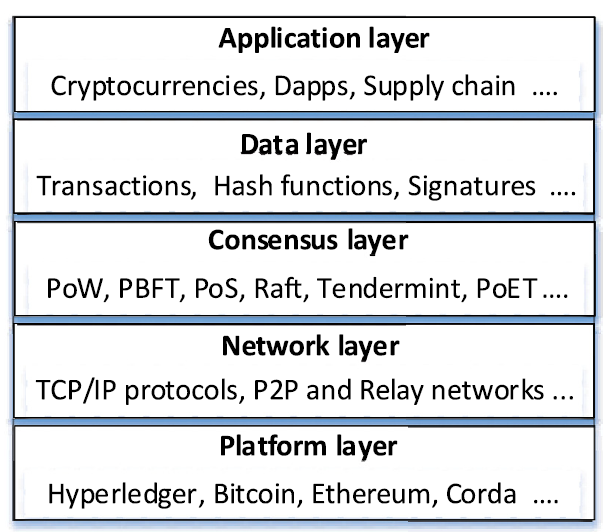
\includegraphics[width=0.90\textwidth]{figures/chapter2/generic_zk_workflow.png}
    \caption{Generic ZK-rollup workflow.}
    \label{fig:zk_workflow}
\end{figure}
\label{sec:rollups}

Rollups work by executing transactions off-chain in a separate environment. A specialized node, called a sequencer, groups many of these off-chain transactions into a single "batch." The sequencer then submits a summary of this batch (including the updated state root and necessary transaction data) to the L1 blockchain.

By grouping transactions, rollups amortize the fixed L1 submission and verification costs across the entire batch, dramatically increasing effective throughput and lowering the cost per transaction.
As illustrated in Figure~\ref{fig:zk_workflow}, a ZK-Rollup batches transactions off-chain and submits a cryptographic proof to the main chain.
